\documentclass{beamer}
\usepackage{boondox-calo} % lowercase calligraphic letters
\usepackage[backend=biber]{biblatex}
\usepackage{optidef}

\beamertemplatenavigationsymbolsempty
\usetheme{Warsaw}
\addbibresource{reference.bib}
\setbeamertemplate{bibliography item}{\insertbiblabel}

%% label
% po=problem objective
% pc=problem constraint

%% miscellaneous
\renewcommand
{\th}
{\textsuperscript{th}}

%% math
\newcommand
{\set}
[1]
{\left\{ #1 \right\}}

\newcommand
{\const}
{\mathfrak}

\renewcommand
{\vec}
[1]
{\boldsymbol{\mathbf{#1}}}

\newcommand
{\dB}
[1]
{#1^{dB}}

\newcommand
{\unit}
[1]
{\left[ #1 \right]}

%% problem
\newcommand
{\numerology}
{\mu}

\newcommand
{\power}
{p}

\newcommand
{\powTx} % transmitted power
{\const{\power}_{tx}}

\newcommand
{\powRx} % received power
[2]
{\power_{rx}(#1, #2)}

\newcommand
{\powRxDB}
[2]
{\power_{rx}^{dB}(#1, #2)}

\newcommand
{\frequency}
{f}

\newcommand
{\freq}
[1]
{\const{\frequency}_{#1}}

\newcommand
{\subcarrierSpacing}
{\zeta}

\newcommand
{\genericSubchannel}
{sc}

\newcommand
{\subchannelBandwidth}
{\const{w}_{\genericSubchannel}}

\newcommand
{\lightSpeed}
{3 \cdot 10^{8}}

\newcommand
{\distance}
{d}

\newcommand
{\pathLoss}
[2]
{h(#1, #2)}

\newcommand
{\pathLossDB}
[2]
{h^{dB}(#1, #2)}

\newcommand
{\pathLossExponent}
{\epsilon_{pl}}

\newcommand
{\shadowingStddv} % shadowing standard deviation
{\sigma_{sd}}

\newcommand
{\cci} % co-channel interference
[1]
{\const{i}_{#1}}

\newcommand
{\subchannelThermalNoise}
{\const{o}_{\genericSubchannel}}

\newcommand
{\utilComp} % utility composite function
[1]
{\ln{#1}}

\newcommand
{\rate}
{r}

\newcommand
{\peakRate}
{\const{\rate}}

\newcommand
{\avgRate} % average rate
[1]
{\bar{\rate_{#1}}}

\newcommand
{\timeDuration}
{\const{t}}

\newcommand
{\timeSlotDuration}
{\timeDuration_{sl}}

\newcommand
{\timeMinislotDuration}
{\timeDuration_{ms}}

\newcommand
{\timeSlot}
{n}

\newcommand
{\timeSlotNum}
{\const{\timeSlot}}

\newcommand
{\timeMinislot}
{m}

\newcommand
{\timeMinislotNum}
{\const{\timeMinislot}}

\newcommand
{\subchannel}
{l}

%% embb macro
\newcommand
{\embbUser}
{u}

\newcommand
{\embbRa} % embb resource allocation
{\alpha}

\newcommand
{\embbVec} % embb vector
{\vec{\embbRa}}

\newcommand
{\embbThree}
[3]
{\embbRa_{#1, #2, #3}}

\newcommand
{\pRateSlot}
[3]
{\peakRate_{#1, #2, #3}}

\newcommand
{\embbDist}
[2]
{\const{\distance}_{#1, #2}}

%% urllc macro
\newcommand
{\urllcUser}
{v}

\newcommand
{\urllcRa} % urllc resource allocation
{\beta}

\newcommand
{\urllcVec} % urllc vector
{\vec{\urllcRa}}

\newcommand
{\urllcFive}
[5]
{\urllcRa_{#1, #2, #3, #4, #5}}

\newcommand
{\rateMinislot}
[3]
{\rate_{#1, #2, #3}}

\newcommand
{\demandRate}
{R}

\newcommand
{\dRateThree}
[3]
{\demandRate_{#1, #2, #3}}

\newcommand
{\pRateMinislot}
[4]
{\peakRate_{#1, #2, #3, #4}}

\newcommand
{\pRateMinislotMin}
[3]
{\peakRate_{#1, #2, #3}}

\newcommand
{\urllcDist}
[3]
{\const{\distance}_{#1, #2, #3}}

\title{Multiplexing URLLC Traffic Within eMBB Services in 5G NR: Fair Scheduling}
\author{Hao Yin, Lyutianyang Zhang, Sumit Roy}
\institute{Department of Electrical and Computer Engineering, University of Washington, Seattle, USA}
\date{February, 2021}

\begin{document}

\begin{frame}
  \titlepage
  Published in IEEE Transactions on Communications
\end{frame}

\begin{frame}
  \frametitle{System Model}
  \begin{itemize}
    \item One base station, downlink transmission, orthogonal frequency-division multiple accses (OFDMA), eMBB and URLLC users.
    \item Saturated eMBB traffic \cite{S05}: Each eMBB user has infinite amount of data to be served.
  \end{itemize}
  \begin{figure}
    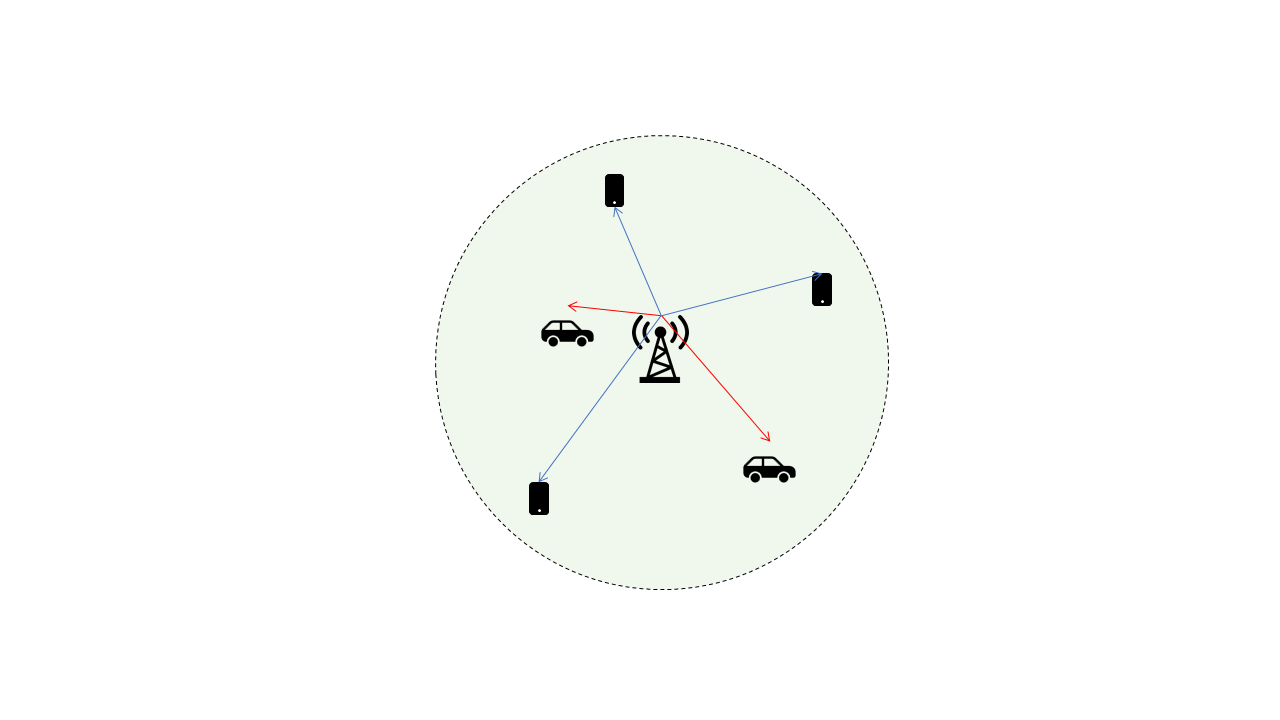
\includegraphics[width=0.7\textwidth]{system_model}
    \caption{System model}
  \end{figure}
\end{frame}

\begin{frame}
  \frametitle{Numerology}
  \begin{itemize}
    \item $\numerology = 2$ for mmWave 28GHz is used ($\numerology \in \set{ 0, 1 }$ is for Sub-6GHz).
    \item Subcarrier spacing
      \begin{equation}
        \subcarrierSpacing = 2^{ \numerology } \cdot 15 \unit{kHz}
      \end{equation}
    \item Subchannel bandwidth
      \begin{align}
        \subchannelBandwidth &= 12 \cdot \subcarrierSpacing &\unit{kHz}\\
        &= 2^{ \numerology } \cdot 180 &\unit{kHz}\\
        &= 720 &\unit{kHz}\\
        &= 7.2 \cdot 10^{ 5 } &\unit{Hz}
      \end{align}
    \item Time slot duration
      \begin{align}
        \timeSlotDuration &= \frac{ 1 }{ 2^{ \numerology } } &\unit{ms}\\
        &= 0.25 &\unit{ms}\\
        &= 2.5 \cdot 10^{ -4 } &\unit{s}
      \end{align}
  \end{itemize}
\end{frame}

\begin{frame}
  \frametitle{Numerology (Continued)}
  \begin{figure}
    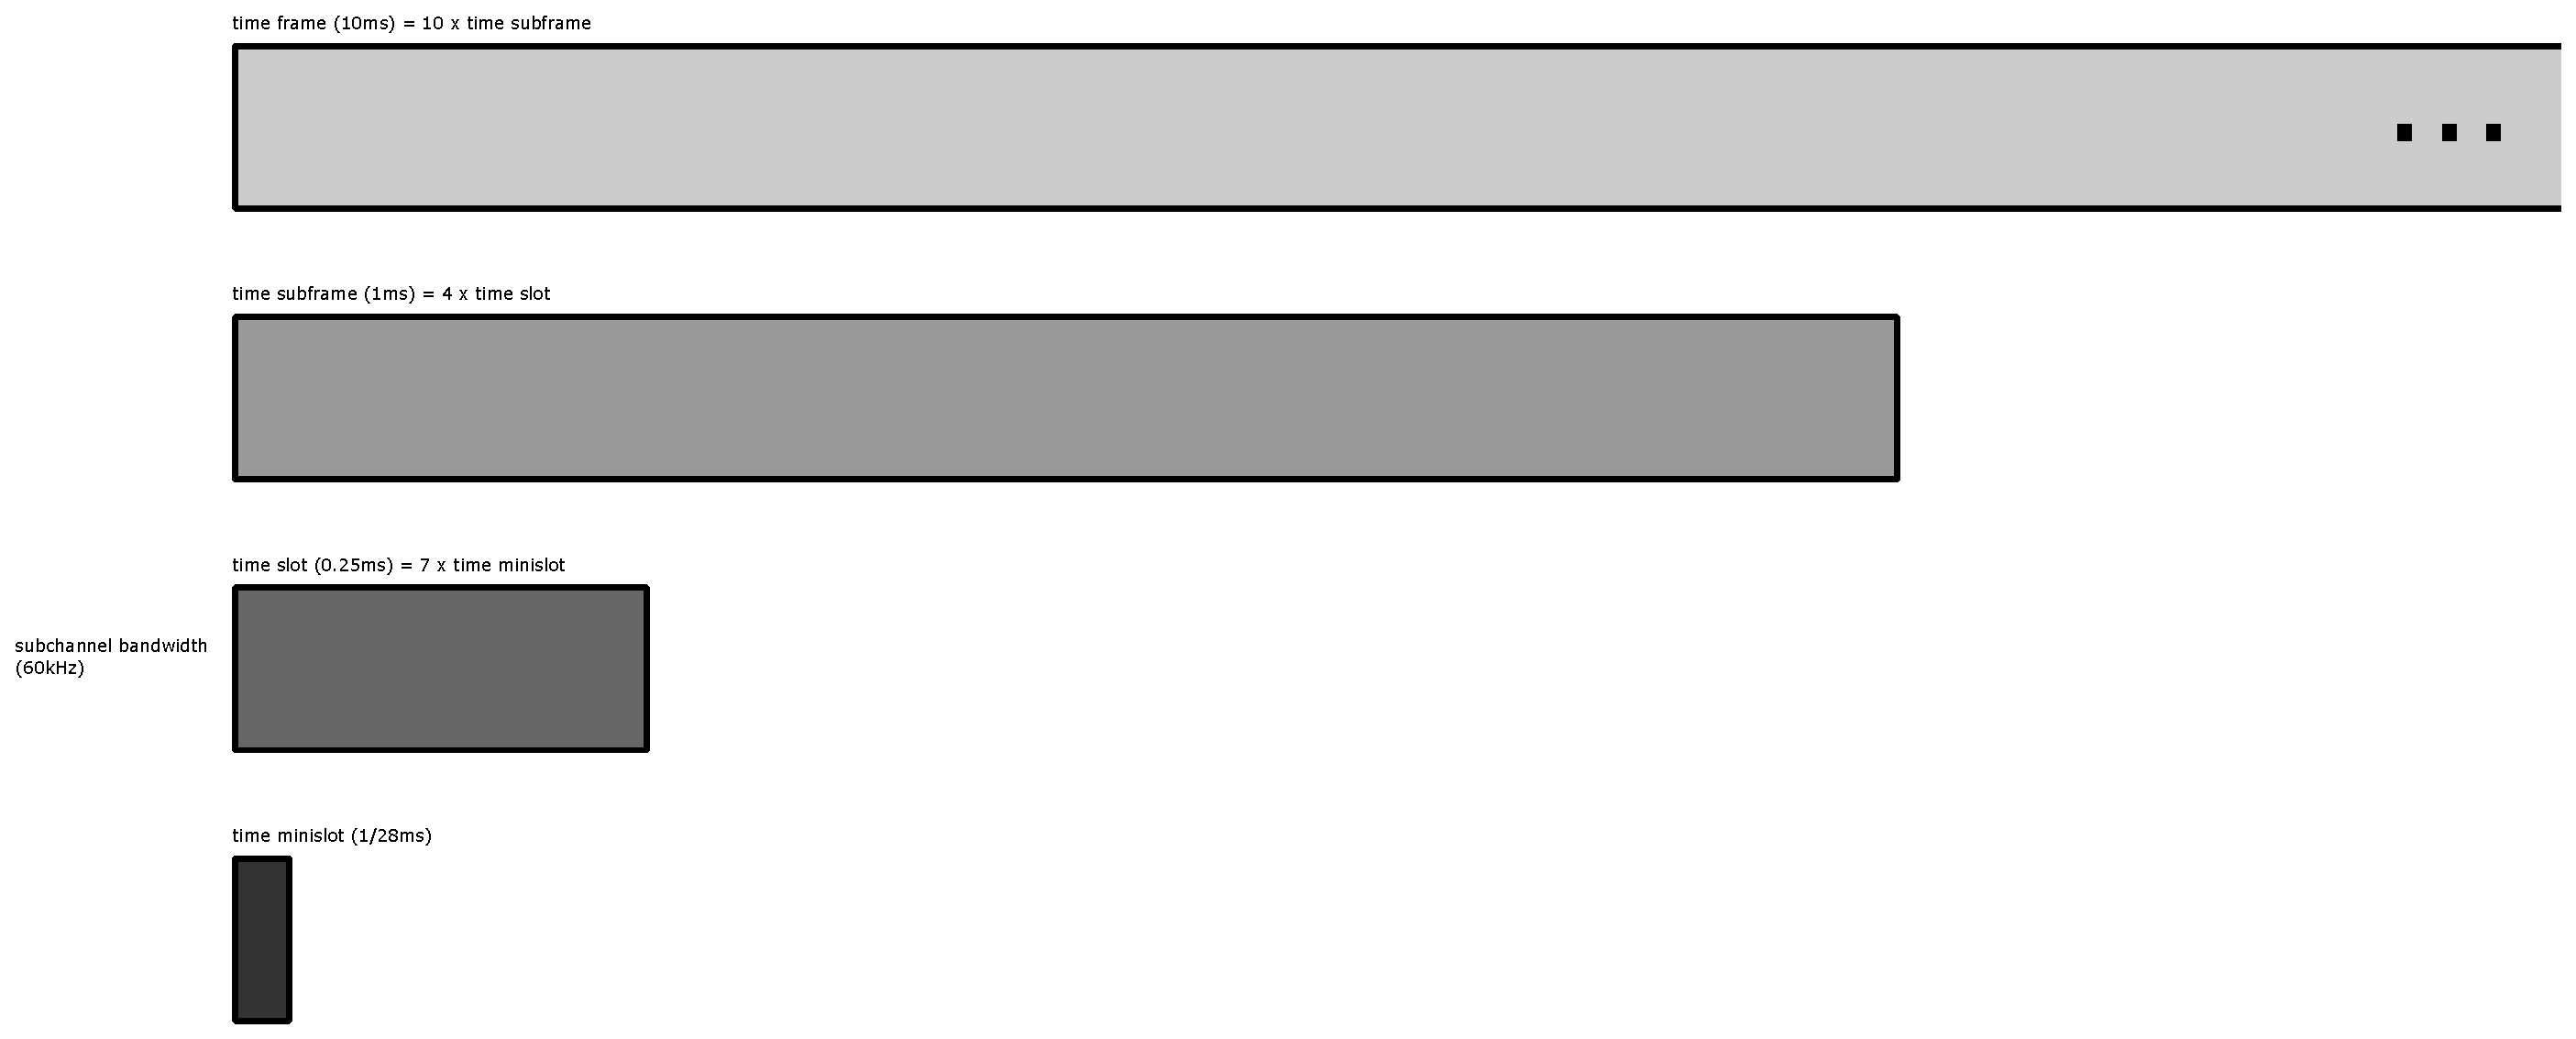
\includegraphics[width=\textwidth]{numerology}
    \caption{Numerology}
  \end{figure}
\end{frame}

\begin{frame}
  \frametitle{System Framework}
  \begin{itemize}
    \item 3 eMBB users $\set{ \textcolor{blue}{0}, \textcolor{yellow}{1}, \textcolor{green}{2} }$.
    \item 2 URLLC users $\set{ \textcolor{orange}{0}, \textcolor{red}{1} }$.
    \begin{figure}
      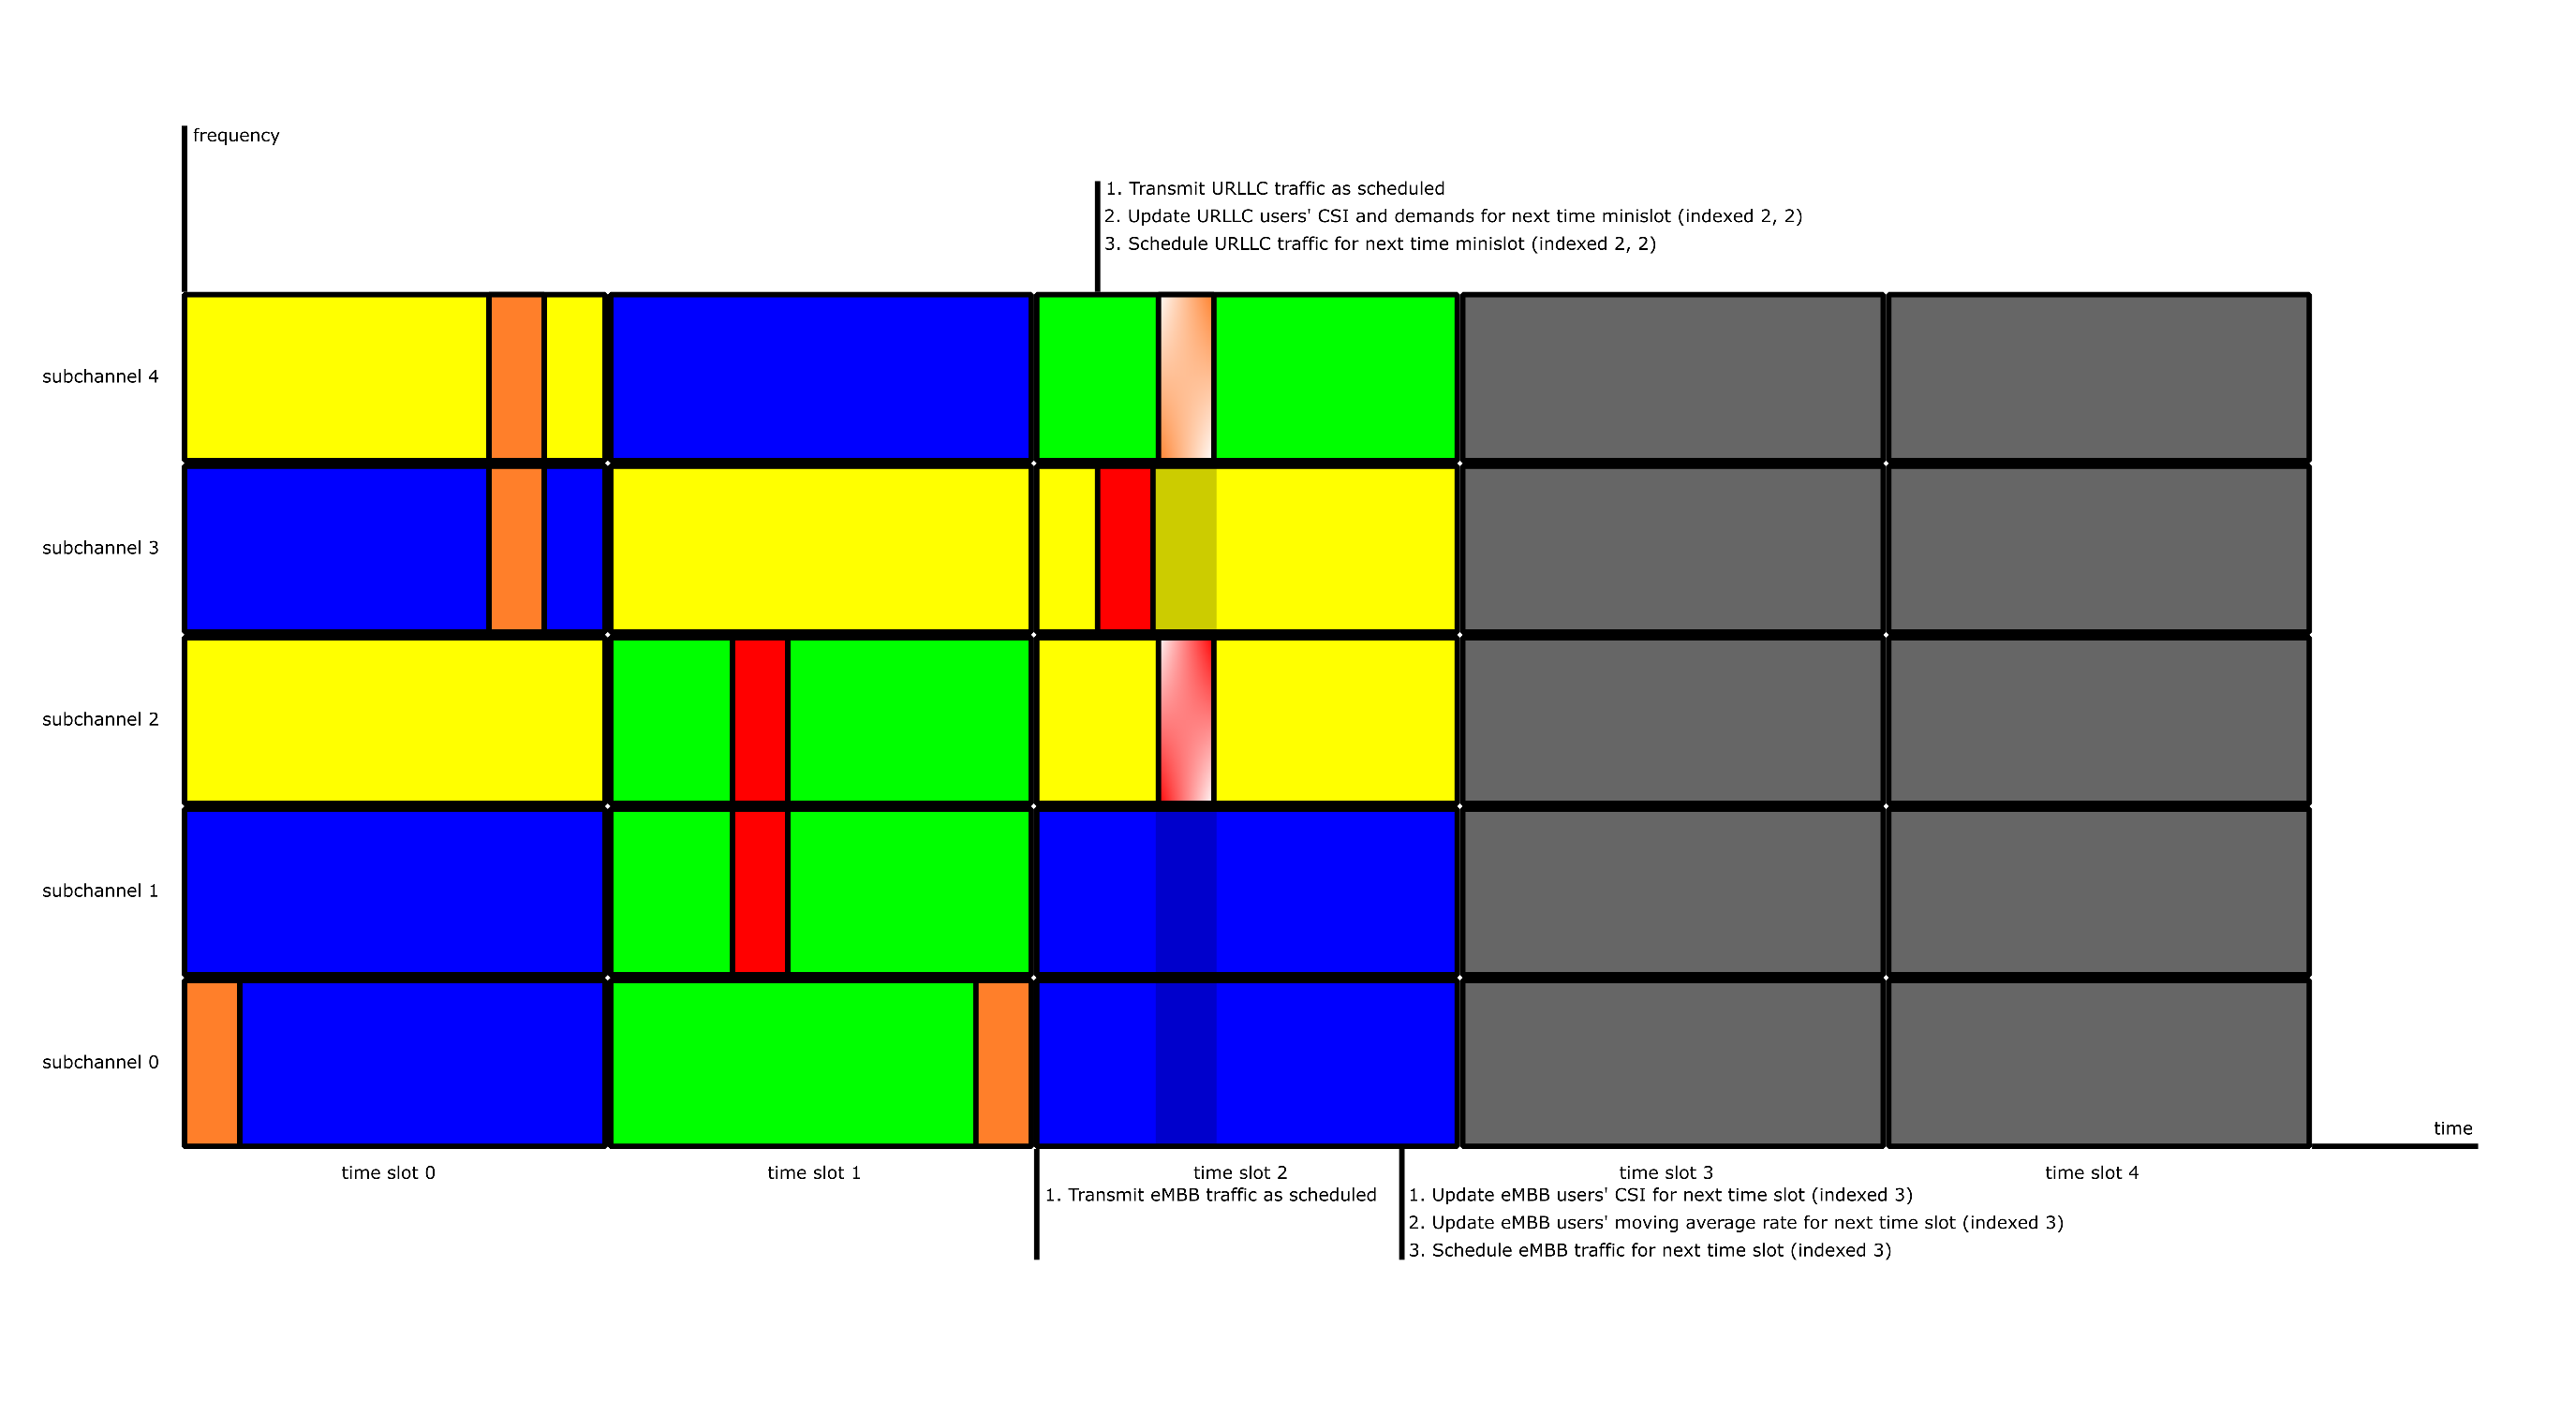
\includegraphics[width=\textwidth]{system_framework}
      \caption{System framework}
    \end{figure}
  \end{itemize}
\end{frame}

\begin{frame}
  \frametitle{Offline URLLC Puncturing}
  \begin{itemize}
    \item The system maximizes eMBB traffic's total average rate and fairness \eqref{po:offline}.
    \item For each time slot, the system allocates at most one eMBB user to each subchannel \eqref{pc:offline1}.
    \item For each time slot, the system either schedules or un-schedules a subchannel to each eMBB user \eqref{pc:offline2}.
    \item For each time minislot, the system allocates at most one URLLC user to each subchannel. Also, it schedules $\subchannel^{th}$ subchannel from $\embbUser^{th}$ eMBB user to a URLLC user only if it schedules the subchannel to the eMBB user \eqref{pc:offline3}.
    \item For each time minislot, the system serves URLLC demands without delay \eqref{pc:offline4}.
    \item For each time minislot, the system employs URLLC puncturing instead of superposition \eqref{pc:offline5}.
  \end{itemize}
\end{frame}

\begin{frame}
  \frametitle{Offline URLLC Puncturing (Continued)}
  \begin{maxi!}
    { \embbVec, \urllcVec }{ \sum_{ \embbUser }{ \utilComp{\avgRate{\embbUser} } } \label{po:offline} }
    {}{}
    \addConstraint
      { \sum_{ \embbUser }{ \embbThree{\embbUser}{\timeSlot}{\subchannel} } }
      { \leq 1,\quad \label{pc:offline1} }
      { \forall\timeSlot, \forall\subchannel }
    \addConstraint
      { \embbThree{\embbUser}{\timeSlot}{\subchannel} }
      { \in \set{ 0, 1 },\quad \label{pc:offline2} }
      { \forall\embbUser, \forall\timeSlot, \forall\subchannel }
    \addConstraint
      { \sum_{ \urllcUser }{\urllcFive{\urllcUser}{\embbUser}{\timeSlot}{\timeMinislot}{\subchannel} } }
      { \leq \embbThree{\embbUser}{\timeSlot}{\subchannel},\quad \label{pc:offline3} }
      { \forall\embbUser, \forall\timeSlot, \forall\timeMinislot, \forall\subchannel }
    \addConstraint
      { \rateMinislot{\urllcUser}{\timeSlot}{\timeMinislot} }
      { \geq \dRateThree{\urllcUser}{\timeSlot}{\timeMinislot},\quad \label{pc:offline4} }
      { \forall\urllcUser, \forall\timeSlot, \forall\timeMinislot }
    \addConstraint
      { \urllcFive{\urllcUser}{\embbUser}{\timeSlot}{\timeMinislot}{\subchannel} }
      { \in \set{ 0, 1 },\quad \label{pc:offline5} }
      { \forall\urllcUser, \forall\embbUser, \forall\timeSlot, \forall\timeMinislot, \forall\subchannel }
  \end{maxi!}
\end{frame}

\begin{frame}
  \frametitle{Offline URLLC Puncturing (Continued)}
  where
  \begin{align}
    \avgRate{\embbUser} &= \frac{ 1 }{ \timeSlotNum } \sum_{ \timeSlot, \timeMinislot, \subchannel }{ \left( \embbThree{\embbUser}{\timeSlot}{\subchannel} - \sum_{ \urllcUser }{ \urllcFive{\urllcUser}{\embbUser}{\timeSlot}{\timeMinislot}{\subchannel} } \right) \frac{ \pRateSlot{\embbUser}{\timeSlot}{\subchannel} }{ \timeMinislotNum } },\quad \forall\embbUser\\
    \rateMinislot{\urllcUser}{\timeSlot}{\timeMinislot} &= \sum_{ \embbUser, \subchannel }{ \urllcFive{\urllcUser}{\embbUser}{\timeSlot}{\timeMinislot}{\subchannel} \pRateMinislotMin{\urllcUser}{\timeSlot}{\timeMinislot} },\quad \forall\urllcUser, \forall\timeSlot, \forall\timeMinislot\\
    \pRateMinislotMin{\urllcUser}{\timeSlot}{\timeMinislot} &= \min_{ \subchannel }{ \left\{ \pRateMinislot{\urllcUser}{\timeSlot}{\timeMinislot}{\subchannel} \right\} },\quad \forall\urllcUser, \forall\timeSlot, \forall\timeMinislot
  \end{align}
\end{frame}

\begin{frame}
  \frametitle{Channel Model -- Path Loss and Shadowing}
  \begin{itemize}
    \item Large-scale propagation path loss model (power in \textcolor{red}{W})
      \begin{align}
        \frac{ \powTx }{ \powRx{\frequency}{\distance} } &= \pathLoss{\frequency}{\distance}\\
        \powRxDB{\frequency}{\distance} &= \dB{\powTx} - \pathLossDB{\frequency}{\distance}
      \end{align}
    \item Close-in (CI) free space reference distance model
      \begin{equation}
        \pathLossDB{\frequency}{\distance} = 20 \log_{ 10 }{ \frac{ 4 \pi \frequency }{ \lightSpeed } } + 10 \pathLossExponent \log_{10}{\distance} + \dB{\shadowingStddv}
      \end{equation}
    \item Path loss exponent and shadowing standard deviation for urban macro-cellular (UMa) line-of-sight (LoS) over frequency and 3D distance ranging from 2 to 73.5\textcolor{red}{GHz} and 58 to 930\textcolor{red}{m} are derived as \cite{SRRTGKRKPJ16}
      \begin{align}
        \pathLossExponent &= 2\\
        \dB{\shadowingStddv} &= 4.6
      \end{align}
  \end{itemize}
\end{frame}

\begin{frame}
  \frametitle{Channel Model -- Co-channel Interference and Thermal Noise}
  \begin{itemize}
    \item Shannon-Hartley theorem (bandwidth in \textcolor{red}{Hz}, time in \textcolor{red}{s})
      \begin{align*}
        \pRateSlot{\embbUser}{\timeSlot}{\subchannel} &= \subchannelBandwidth \log_{ 2 }{ \left( 1 + \frac{ \powRxDB{\freq{\subchannel}}{\embbDist{\embbUser}{\timeSlot}} }{ \dB{\cci{\subchannel}} + \dB{\subchannelThermalNoise} } \right) } \timeSlotDuration \unit{\frac{ bits }{ slot }},\quad\\
          &\forall\embbUser, \forall\timeSlot, \forall\subchannel\\
        \pRateMinislot{\urllcUser}{\timeSlot}{\timeMinislot}{\subchannel} &= \subchannelBandwidth \log_{ 2 }{ \left( 1 + \frac{ \powRxDB{\freq{\subchannel}}{\urllcDist{\urllcUser}{\timeSlot}{\timeMinislot}} }{ \dB{\cci{\subchannel}} + \dB{\subchannelThermalNoise} } \right) } \timeMinislotDuration \unit{\frac{ bits }{ minislot }},\quad\\
          &\forall\urllcUser, \forall\timeSlot, \forall\timeMinislot, \forall\subchannel
      \end{align*}
    \item where
      \begin{equation}
        \timeMinislotDuration = \frac{ \timeSlotDuration }{ \timeMinislotNum }
      \end{equation}
    \item Channel fading and inter-symbol interference (ISI) are not considered.
  \end{itemize}
\end{frame}

\begin{frame}
  \frametitle{References}
  \printbibliography[heading=none]
\end{frame}

\end{document}
